%Optical waveguides
For the transmission of optical signal optical waveguides are applied. The general waveguides are semiconductor waveguide and optical fibers. 
Fig. \ref{fig:semi_waveguides} shows two semiconductor waveguides commonly used in integrated optics. Rib waveguide is composed of a rib guide on a substrate ($n=n_{2}$). Buried waveguide is a high index guide ($n=n_{1}$) surrounded by low index cladding ($n=n_{2}$).\\
\begin{figure}
\centering
\subfigure[Rib waveguide]{
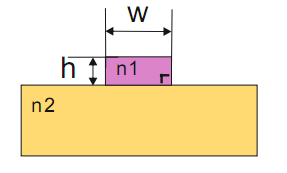
\includegraphics[width=0.4\textwidth]{bilder/approxmate_waveguide}
\label{fig:semi_rib_waveguide}
}
\hfill
\subfigure[Buried waveguide]{
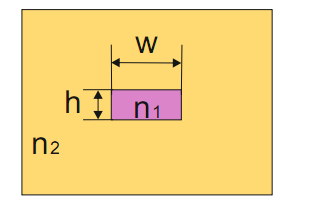
\includegraphics[width=0.4\textwidth]{bilder/buried_waveguide}
\label{fig:semi_buried_waveguide}
}
\caption{Schema of semiconductor waveguides}
\label{fig:semi_waveguides}
\end{figure}
Optical fibers are widely used for telecommunication and data networks. The Fig.\ref{fig:opticfiber} presents a simplest optical fiber and how lights propagate in the fiber . Optical fiber typically consists of a transparent core with index $n_{1}$ surrounded by a transparent cladding material with a lower index of refraction $n_{2}$. 


\begin{figure}[httbp]
\centering
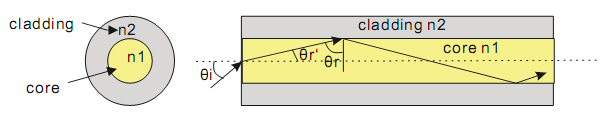
\includegraphics[width=0.8\textwidth]{bilder/opticfiber}
\caption{linght refraction in optic fibers}
\label{fig:opticfiber}
\end{figure}
\textbf{ Total Reflection}\\
\begin{figure}[!ht]
\centering
\subfigure[totalreflection]{
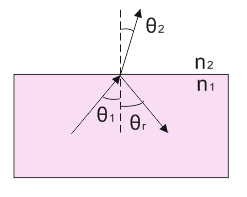
\includegraphics[width=0.3\textwidth]{bilder/totalreflection01}
\label{fig:totalreflection01}
}
\hfill
\subfigure[Buried waveguide]{
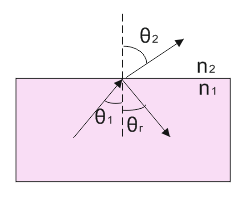
\includegraphics[width=0.3\textwidth]{bilder/totalreflection02}
\label{fig:totalreflection02}
}
\hfill
\subfigure[Buried waveguide]{
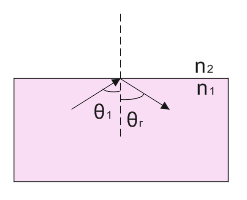
\includegraphics[width=0.3\textwidth]{bilder/totalreflection03}
\label{fig:totalreflection03}
}
\caption{Total reflection}
\label{fig:totalreflection}
\end{figure}

Whatever semiconductor waveguides or optical fibers, the principle of the light propagation in waveguides is total reflection. The principle of the total reflection is explained in \cite{optical_waveguides_fibers} with Snell's law. In Fig.\ref{fig:totalreflection01} the input light strikes the boundary between two different isotropic media with respective refractive index $n_{1}$ and $n_{2}$. Where $theta_{1}$ is incidence angle, $\theta_{2}$ refractive angle and $\theta_{r}$ reflective angle. Through SNELL's Law there are relations (\ref{eq:snell}-\ref{eq:reflection}).  For $n_{1}<n_{2}$ there is  always a relation $\theta_{1}>\theta_{2}$.  If the refractive indexes has the relation $n_{1}>n_{2}$, then the incidence angle $\theta_{1}$ is narrower than the refractive angle $\theta_{2}$ like Fig. \ref{fig:totalreflection02}. If the incidence angle is increased wider than a critical angle $\theta_{c}$ (\ref{eq:critical_angle}) there will be no light passing through the boundary and all of the lights are reflected like Fig. \ref{fig:totalreflection03}. This phenomenon is so called total reflection.
\begin{align}
n_{1}sin\theta_{1}&=n_{2}sin\theta_{2}
\label{eq:snell}\\
\theta_{1}=\theta{r}
\label{eq:reflection}
\end{align}
\begin{equation}
\theta_{c}=arcsin(\frac{n_{2}}{n_{1}})
\label{eq:critical_angle}
\end{equation}
%%dispersion
\textbf{ Numerical Apertur }\\
%Numerical Aperture
Another important character of optical waveguides is numerical aperture. Back to the Fig.\ref{fig:opticfiber} the incidence beam originate from the air into the fiber. There is a maximum coupling angle, so that the beam can be guided under the total reflecting conditions. Its sinus value (\ref{eq:NA}) is called \textbf{Numerical Apertur(NA)}, which indicate the acceptable range of ray beams.
\begin{align}
sin\theta_{i}&=\frac{n_{1}}{n_{0}}sin(90^{o}-\theta_{c})=n_{1}cos\theta_{c} \nonumber\\
&=n_{1}\sqrt{1-sin^{2}\theta_{c}}=n_{1}\sqrt{1-\left(\frac{n_{2}}{n_{1}}\right)^2}=\sqrt{n^2_{1}-n^2_{2}}
\label{eq:NA}
\end{align}
\textbf{Mode of the waveguide}\\
"' An eigenmode $m$ of a waveguide structure is a propagation or evanescent wave which maintains its transverse shape during propagation "'\cite{integrated_optics}. The eigenmode of a waveguide can be presented as (\ref{eq:e_eigenmode}-\ref{eq:h_eigenmode}). 
\begin{align}
E^{m}(r_{t},z)&=E^{m}_{0}(r_{t})e^{jk_{m}z}
\label{eq:e_eigenmode}\\
H^{m}(r_{t},z)&=H^{m}_{0}(r_{t})e^{jk_{m}z}
\label{eq:h_eigenmode}
\end{align}
Where $k_{m}$ is the propagation constant. When the request  $k_{0}n_{1}>k_{m}>k_{0}n_{2}$ is matched this mode is a guided mode for the waveguides \cite{script_FT_TET}. In this work the coupling bases on the fundamental mode.
